\documentclass[11pt,letterpaper,twoside,english]{article}

\usepackage[margin=1.4in]{geometry} % controls the size of the margins

% Special symbols, etc.
\usepackage{amssymb,amsbsy,latexsym}
\usepackage{amsmath}
\usepackage{graphics, subfigure, float} 
\usepackage{cancel}
%\usepackage{todonotes}
% Encoding settings
\usepackage[latin1]{inputenc}
\usepackage[american]{babel}
\usepackage[T1]{fontenc} 

\usepackage{titling} % allows posttitle command

% AMS Math packages

\usepackage{amscd,amsthm}

\usepackage{verbatim, comment} % can comment out text 
\usepackage{mdwlist} 

% Graphics
\usepackage[dvips]{graphicx,epsfig,color}
\usepackage{subfigure}
%\usepackage{pst-all}
%\usepackage{pstricks-add}
\usepackage{hyperref}  % can only be used with pdflatex - gives hyperlinks
\usepackage{bm} % bold math font
\usepackage{bbm}
\usepackage{todonotes}

\newtheoremstyle{theorem}{1em}{1em}{\slshape}{0pt}{\bfseries}{.}{ }{}
\theoremstyle{theorem}
\newtheorem{theorem}{Theorem}
\newtheorem*{theorem*}{Theorem}
\newtheorem{corollary}[theorem]{Corollary}
\newtheorem{proposition}[theorem]{Proposition}
\newtheorem{lemma}[theorem]{Lemma}
\newtheorem{claim}[theorem]{Claim}
\newtheorem{conjecture}[theorem]{Conjecture}
\newtheorem{definition}[theorem]{Definition}
\newtheorem*{claim*}{Claim}

\theoremstyle{remark}
\newtheorem{remark}{Remark}
\newtheorem*{remark*}{Remark}
\newtheorem{algorithm}{Algorithm}
\newtheorem*{question*}{Question}
\newtheorem{question}{Question}
\newtheorem{example}{Example}

\providecommand{\setN}{\mathbb{N}}
\providecommand{\setZ}{\mathbb{Z}}
\providecommand{\setQ}{\mathbb{Q}}
\providecommand{\setR}{\mathbb{R}}
\providecommand{\E}{\mathrm{E}}
\providecommand{\Pr}{\mathrm{Pr}}
\providecommand{\Var}{\mathrm{Var}}

\makeatother

\title{Greedy sequences of integers} 

\author{Yajit Jain, Deepak Narayanan, Leon Zhang}

\begin{document}

\maketitle

\section{Introduction} \label{sec:intro}

In this paper, we look at the sequence of integers $A=(a_i)_{i\in\mathbb{Z}_{\ge 0}}$ defined inductively as follows. 

\begin{definition} \label{def:seqA}
The sequence $A$ is defined as the sequence of numbers $a_0, a_1, a_2, \ldots$ such that $a_0 = 0$, and all subsequent terms $a_{n}$ are defined as the least term greater than $a_{n-1}$ such that no three distinct terms in the set $\{a_0, a_1, a_2, \ldots, a_n\}$ form a $3$-term arithmetic progression.
\end{definition}

It turns out that this sequence $A$ has a number of extremely interesting properties. We state and prove some of these conjectures below.

Before we begin, consider the beginning of the sequence $A$. All numbers less than 40 that are not in the sequence have been crossed out.

\

\noindent 0, 
\\1, \xcancel2,
\\3, 4, \xcancel5, \xcancel6, \xcancel7, \xcancel8,
\\9, 10, \xcancel{11}, 12, 13, \xcancel{14}, \xcancel{15}, \xcancel{16}, \xcancel{17}, \xcancel{18}, \xcancel{19}, \xcancel{20}, \xcancel{21}, \xcancel{22}, \xcancel{23}, \xcancel{24}, \xcancel{25}, \xcancel{26},
\\27, 28, \xcancel{29}, 30, 31, \xcancel{32}, \xcancel{33}, \xcancel{34}, \xcancel{35}, 36, 37, \xcancel{38}, 39, 40

 
 \
 
The terms above are formatted to draw attention to a very specific pattern: all powers of $3$ less than $a_{15}=40$ appear in the sequence. This observation is at the heart of many of the results we shall prove about this sequence and its variants. The main result regarding the sequence $A$ is stated below and proven in Section \ref{sec:AP}. In what follows $(\cdot)_3$ will denote the base three expansion, and $(\cdot)_2$ will denote the base two expansion. 


\

 {\itshape If the binary representation of $n$ is $(b_kb_{k-1}\ldots b_0)_2$, where $b_0, b_1, b_2, \ldots, b_k \in \{0, 1\}$, then $a_n = (b_k b_{k-1}\ldots b_0)_3.$}

\

In Sections \ref{sec:GP}, \ref{sec:firstTerm}, and \ref{sec:diffEquation}, we consider variations of this sequence $A$. First we consider the problem of avoiding geometric sequences of length 3. We will show that the problem of avoiding 3-term geometric sequences is very closely related to the problem of avoiding 3-term arithmetic sequences, and the closed form of the sequence $A$ can be used to characterize the geometric progression avoiding sequence $G$. 

In Section \ref{sec:firstTerm}, we will show that the behavior of the sequence $A$ is heavily dependent on the initial conditions of the sequence. In particular, if we let $a_0=0$ and $a_1=m$, the sequence is significantly altered. 

Finally, we note that avoiding three-term arithmetic progressions is equivalent to the problem of avoiding triplets $x,y,z\in S$ that are solutions to the equation $x+z=2y$. In Section \ref{sec:diffEquation}, we consider the problem of avoiding solutions to the equation $x+z =y$.



\emph{Yajit wrote and edited this section. Leon made close edits to this section. Deepak edited this section.}

\section{Avoiding three-term arithmetic progressions} \label{sec:AP}

As motivation, notice that the number preceding any number of the form $3^n$ in $A$ is exactly $\frac{3^n-1}{2}$. This can be factored as 
\[\frac{3^n-1}{2}=\frac{(3-1)(3^{n-1}+3^{n-2}+\ldots+3+1)}{(3-1)}=3^{n-1}+3^{n-2}+\ldots+3+1,\]
which is the sum of all smaller powers of $3$.

Also notice that if we consider the entries of each row modulo the power of $3$ at the beginning of the row, the sequence appears to regenerate itself:

\

\noindent 0, 
\\0, 
\\0, 1, 
\\0, 1, 3, 4, 
\\ 0, 1, 3, 4, 9, 10, 12, 13,
\\0, 1, 3, 4, 9, 10, 12, 13, 27, 28, 30, 31, 36, 37, 39, 40

 
 \

This recurrence is the motivating example for our first claim. Informally stated, this claim is that the base $3$ representation of each element in the sequence $A$ contains only $0$'s and $1$'s. Once this claim is proven, we can conveniently write a closed form expression for each $a_n\in A$.


%As we observed in the introduction, the sequence $A$ seems to contain all powers of $3$. Furthermore, the preceding term to a power of $3$ seems to be the sum of all smaller powers of 3. Our main result of this section implies that this is true, and more generally characterizes all terms of the sequence.

\begin{definition} \label{def:S_A}
$S_A$ is defined to be the set of integers greater than or equal to zero, of the form $\alpha_k \cdot 3^k + \alpha_{k-1} \cdot 3^{k-1} + \alpha_{k-2} \cdot 3^{k-2} + \ldots + \alpha_1 \cdot 3 + b_0$ where $\alpha_k, \alpha_{k-1}, \alpha_{k-2}, \ldots, \alpha_1, \alpha_0 \in \{0, 1\}$ (that is, all numbers whose representation in base $3$ consists of only $0$s and $1$s). 
\end{definition}

Before proving our main result for this section, we first consider a lemma, which will be of use both in the proof of our main theorem and in future sections.


\begin{lemma} \label{lemma1}
Let $n$ a positive integer such that $n\not\in S_A$. Then there exist specific $\ell, m\in S_A$ whose base $3$ representations are $(\ell_k \ell_{k-1}\dots \ell_0)_3$ and $(m_km_{k-1}\ldots m_0)_3$ such that $\ell, m, n$ is a strictly increasing arithmetic progression and, for each $0\leq i \leq k$, either $\ell_i=m_i$ or $\ell_i=0, m_i=1$. Furthermore, for each $i$ such that $\ell_i=m_i$, the $i^{th}$ digit of the base 3 representation of $n$ is also $\ell_i$. For each $i$ such that $\ell_i=0, m_i=1$, the $i^{th}$ digit of the base 3 representation of $n$ is $2$.
\end{lemma}
\begin{proof}
Because $n$ does not belong to $S_A$, its base 3 representation contains at least one 2. We can therefore express $n$ as
\[n=2\cdot (3^{y_1}+3^{y_2}+\ldots + 3^{y_i})+n_{x_1}\cdot 3^{x_1}+n_{x_2}\cdot 3^{x_2}+\ldots+n_{x_j}\cdot 3^{x_j}\]
where the exponents are pairwise distinct, and each $x_1,\ldots, x_j\in \{0,1\}$. (In essence, we are separating the powers of 3 with digit 2 in the base 3 representation of $n$ from the powers of 3 with digit either 0 or 1)

Define $\ell$ as
\[\ell=0\cdot (3^{y_1}+3^{y_2}+\ldots + 3^{y_i})+n_{x_1}\cdot 3^{x_1}+n_{x_2}\cdot 3^{x_2}+\ldots+n_{x_j}\cdot 3^{x_j}\]
and $m$ as
\[m=1\cdot (3^{y_1}+3^{y_2}+\ldots + 3^{y_i})+n_{x_1}\cdot 3^{x_1}+n_{x_2}\cdot 3^{x_2}+\ldots+n_{x_j}\cdot 3^{x_j}.\]
Clearly, $\ell$ and $m$ have all digits in their base 3 representation equal to 0 or 1, so $\ell, m\in S_A$. It is also plain to see that $\ell, m, n$ form a strictly increasing arithmetic progression. Finally, it is clear by construction that $\ell,m,$ and $n$ satisfy the properties specified in the statement of the lemma.
\end{proof}

\begin{theorem} \label{thm:mainThmA}
The set $S_A$ and the sequence $A$ have the same elements, that is $S_A = A$. If the binary representation of $n$ is $(b_kb_{k-1}\ldots b_0)_2$, where $b_k, b_{k-1}, \ldots, b_0 \in \{0, 1\}$, then $a_n$ is given by the expression
$a_n = (b_k b_{k-1} \ldots b_0)_3.$

\end{theorem}

\begin{proof}
We prove this theorem by induction.

We have two base cases, $0$ and $1$. These numbers have base $3$ representations $(0)_3$ and $(1)_3$, respectively, and both numbers are in $A$: $0$ by definition, and $1$ because it does not form an arithmetic progression with $0$ alone.

Now we prove the inductive case. Let us assume that all numbers up to $n-1$ satisfy the inductive hypothesis: that is, all numbers up to $n-1$ in $S_A$ are in $A$, and all numbers up to $n-1$ not in $S_A$ are {not} in $A$.

We need to show that the inductive hypothesis holds for $n$ as well. There are two simple cases that need to be considered.

\begin{itemize}

\item \textbf{Case 1:} $n \in S_A$

We write $n = n_k \cdot 3^k + n_{k-1} \cdot 3^{k-1} + n_{k-2} \cdot 3^{k-2} + \ldots + n_1 \cdot 3 + n_0$, where each $n_i \in \{0, 1\}$. 

We need to prove that $n$ is a part of the sequence: that is, $n$ does not form a strictly increasing arithmetic progression with any two existing terms in the sequence. 

For the sake of contradiction, assume otherwise. Then $n$ must form a strictly increasing arithmetic progression with two other terms that already exist in the sequence. Let the larger of these two terms be $m$, and let the smaller be $\ell = \ell_k \cdot 3^k + \ell_{k-1} \cdot 3^{k-1} + \ell_{k-2} \cdot 3^{k-2} + \ldots + \ell_1 \cdot 3 + \ell_0$. By our induction hypothesis, we see that the base 3 representation of $\ell$ must consist of only 0's and 1's; that is, each $\ell_i\in\{0,1\}$. Similarly, we see that the base 3 representation of $m$ also consists of only 0's and 1's.

Note that $\ell, m, n$ being a strictly increasing arithmetic progression implies that $\ell+n=2m$. Since each digit of the base 3 representation of $m$ is either 0 or 1, we see that each of the terms $(n_k + \ell_k), (n_{k-1} + \ell_{k-1}), \ldots, (n_1 + \ell_1), (n_0 + \ell_0)$ must equal either $0$ or $2$ (since they must equal $2 \cdot m_i$ where $m_i \in \{0, 1\}$). Because each $n_i$ and $\ell_i$ equals either 0 or 1, it follows that for all $i$, we have $n_i=\ell_i$. But then $\ell=n$, a contradiction as $\ell, m, n$ are all distinct by assumption. Hence such an arithmetic progression cannot exist, and it follows that $n\in A$, as desired.
\end{itemize}

\begin{itemize}
\item \textbf{Case 2:} $n \not \in S_A$

From Lemma \ref{lemma1}, we see that we can obtain $\ell, m\in S_A$ such that $\ell, m, n$ is a strictly increasing arithmetic progression. By the inductive hypothesis, $\ell, m$ are also in $A$. Hence $n$ is not an element of $A$, as desired.
\end{itemize}

Since we have checked the inductive hypothesis for both possibilities for $n$, it follows by induction that $S_A=A$. 

Now, since the sequence is monotonically increasing, we see that $a_0 = (0)_3$, $a_1 = (1)_3$, $a_2 = (10)_3$, $a_3 = (11)_3$ and so on.

Observe that $0 = (0)_2$, $1 = (1)_2$, $2 = (10)_2$, $3 = (11)_2$ and so on. Combining the above two facts, we obtain the following closed form expression for $a_n$. If the binary representation of $n$ is $(b_k b_{k-1} \ldots b_0)_2$, where $b_k, b_{k-1}, \ldots, b_0 \in \{0, 1\}$, then $a_n$ is equal to
$$a_n = (b_k b_{k-1} \ldots b_0)_3.$$
That is, the base 3 representation of $a_n$ is the same sequence of $0$'s and $1$'s as $n$ in binary.

\end{proof}

\emph{Leon rewrote parts of the proof and made close edits to this section. Yajit wrote parts of this section and made close edits. Deepak wrote parts of this section, and edited closely.}
\section{Avoiding three-term geometric progressions} \label{sec:GP}

It is natural to ask if there are simple variations of the sequence $A$ with similarly nice closed form expressions for the $n^{\text{th}}$ term. For instance, instead of avoiding three-term arithmetic progressions, what if we avoided three-term geometric progressions instead? 

We now consider the problem of avoiding geometric progressions of length $3$. As it turns out, this problem is closely related to our original problem. Before we proceed further, however, let us formally define this new sequence $G$.

\begin{definition} \label{def:seqG}
$G$ is defined as the sequence of numbers $g_0, g_1, g_2, \ldots$ such that $g_0 = 1$, and all subsequent terms $g_{n+1}$ are defined as the least term greater than $g_n$ such that no three distinct terms in the sequence including $g_{n+1}$ form a geometric progression.
\end{definition}

Here are the first one hundred terms of $G$: 

\

1, 2, 3, 5, 6, 7, 8, 10, 11, 13, 14, 15, 16, 17, 19, 21, 22, 23, 24, 26, 27, 29, 30, 31, 33, 34, 35, 37, 38, 39, 40, 41, 42, 43, 46, 47, 48, 51, 53, 54, 55, 56, 57, 58, 59, 61, 62, 65, 66, 67, 69, 70, 71, 73, 74, 77, 78, 79, 80, 81, 82, 83, 85, 86, 87, 88, 89, 91, 93, 94, 95, 97, 101, 102, 103, 104, 105, 106, 107, 109, 110, 111, 112, 113, 114, 115, 118, 119, 120, 122, 123, 125, 127, 129, 130, 131, 133, 134, 135, 136.

\

While this sequence lacks a pattern as distinguished as the pattern involving powers of three in $A$, we notice that {\itshape{most}} integers appear in this sequence. Indeed, if we plot this sequence and compare it to a plot of the sequence $A$, we see that $A$ grows much faster. 


\begin{figure}[!h]
  \centering
    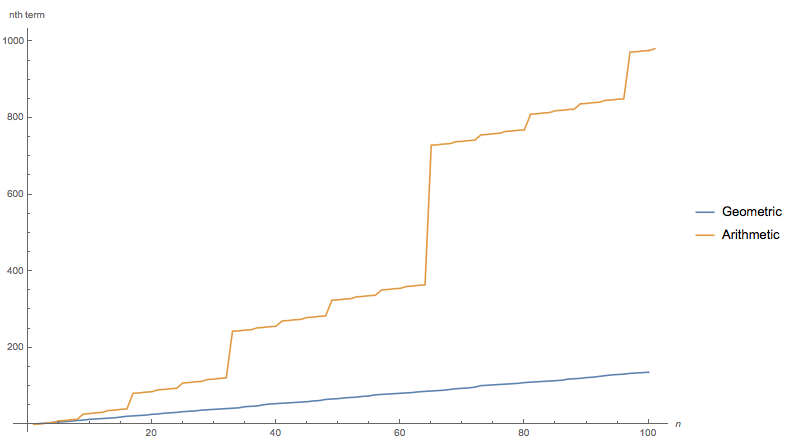
\includegraphics[resolution=120]{GvsS.png}
    \caption{A plot of $a_n$ and $g_n$ versus $n$. Clearly $A$ grows much faster than $G$}
\end{figure}


In this case it is interesting to observe which integers do not appear in this sequence. In particular, the integers 

\

4, 9, 12, 18, 20, 25, 28, 32, 36, 44, 45, 49, 50, 52, 60, 63, 64, 68, 72, 75, 76, 84, 90, 92, 96, 98, 99, 100, 108, 116, 117, 121, 124, 126, 128, 132

\

do not appear in the sequence. If we present the prime factorizations of these numbers we notice a few patterns.

$$
2^2, 3^2, 2^3\cdot 3, 2\cdot3^2, 2^2\cdot 5, 5^2, 2^2\cdot7, 2^5, 2^2\cdot 3^2,\cdots
$$

First, note that squares of primes don't occur in the sequence. It is easy to see why: 1 is in the sequence, and any prime $p$ should appear in the sequence since $p$ cannot be written as a product of smaller integers, and therefore $p$ cannot be in a geometric progression. It then follows that no $p^2$ can be in the sequence. 

In fact, if we ask what powers of $p$ can appear in the sequence, we quickly realize that to avoid geometric progressions in the powers of a single prime we must avoid arithmetic progressions in the exponents of the prime. It is now clear why the original arithmetic sequence in Section \ref{sec:AP} is so crucial to the geometric sequence problem.

This discussion motivates the following theorem. Before stating the theorem, we first define the set $S_G$.
\begin{definition} \label{def:S_G}
$S_G$ is defined to be set of positive integers that have a prime factorization of the form $p_1^{a_1} p_2^{a_2} \ldots p_k^{a_k}$ where $p_1, p_2, \ldots, p_k$ are distinct primes and $a_1$, $a_2$, \ldots, $a_k$ are elements of the sequence $A$.
\end{definition}

\begin{theorem} \label{thm:mainThmG}
 The set $S_G$ and the sequence $G$ have the same elements, that is $S_G=G$. 
\end{theorem}

\begin{proof}
We prove this result using induction. Our inductive hypothesis is that all numbers $i \leq k$ of the form described above (that is, all integers $i \leq k$ in the set $S_G$) belong to the sequence $G$, and that all numbers not of this form (that is, all integers $i \leq k$ not in the set $S_G$) do not belong to the sequence $G$.

Our base case is $k = 2$. $2$ has a prime factorization of $2^1$, and hence is clearly in $S_G$. $1$ and $2$ are also both part of the sequence $G$, since no three-term geometric progression can be formed from $1$ and $2$.

Now, let us assume that the inductive hypothesis holds up to some $k-1$. We want to prove the inductive hypothesis holds for $k$ as well.

Let us factor $k$ as $p_1^{\alpha_1} p_2^{\alpha_2} \ldots p_n^{\alpha_n}$ where $p_1, p_2, \ldots, p_n$ are distinct primes. We consider the following two cases.

\begin{itemize}

\item \textbf{Case 1:} $\alpha_1$, $\alpha_2$, \ldots, $\alpha_n$ are elements of the sequence $A$.

In this case, we want to prove that $k$ is a part of the sequence $G$, that is $k$ does not form a geometric progression with any two $\ell$ and $m$ already in $G$.

Suppose for the sake of contradiction that there exist $\ell, m\in G$ strictly less than $k$ such that $\ell, m, k$ is a three-term geometric progression. Let $\ell = p_1^{\beta_1} p_2^{\beta_2} \ldots p_n^{\beta_n}$ and let $m = p_1^{\gamma_1} p_2^{\gamma_2} \ldots p_n^{\gamma_n}$. Note that some of the $\alpha_i$'s, $\beta_i$'s and $\gamma_i$'s may be equal to $0$, but we do \emph{not} allow $\alpha_i = \beta_i = \gamma_i = 0$ for any $i \in \{1,2,\ldots,n\}$.

Now, by the inductive hypothesis, all the $\beta_i$'s and $\gamma_i$'s are members of the sequence $A$ (including the $0$'s). In addition we just assumed that all the $\alpha_i$'s are members of the sequence $A$ as well.

Without loss of generality, let $\ell < m$. Since $\ell$, $m$ and $k$ form a three-element geometric progression, we see that $\ell \cdot k$ must equal $m^2$. This is equivalent to saying,
$$(p_1^{\beta_1} p_2^{\beta_2} \ldots p_n^{\beta_n}) \cdot (p_1^{\alpha_1} p_2^{\alpha_2} \ldots p_n^{\alpha_n}) = (p_1^{\gamma_1} p_2^{\gamma_2} \ldots p_n^{\gamma_n})^2$$

By comparing the exponents of primes on the left and right sides of the above expression, we obtain the following system of equations that need to hold,

\begin{align}
\alpha_1 + \beta_1 & = 2 \gamma_1 \nonumber \\
\alpha_2 + \beta_2 & = 2 \gamma_2 \nonumber \\
&\mathrel{\makebox[\widthof{=}]{\vdots}} \nonumber \\
\alpha_n + \beta_n & = 2 \gamma_n \nonumber
\end{align}

But note that $\alpha_i$, $\beta_i$ and $\gamma_i$ are members of the sequence $A$, so it is impossible for each of these equations to hold unless $\alpha_i = \beta_i = \gamma_i$. But if for all $i \in \{1, 2, \ldots, n\}$, $\alpha_i = \beta_i = \gamma_i$, then $\ell = m = k$, which is impossible since $\ell$ and $m$ were strictly less than $k$. Therefore by induction $S_G\subseteq G$. 

\item \textbf{Case 2:} At least one of $\alpha_1$, $\alpha_2$, \ldots, $\alpha_n$ is not an element of the sequence $A$.

In this case, we want to prove that $k$ is not an element of the sequence $G$, that is, $k$ forms a three-element geometric progression with some distinct $\ell$ and $m$, where $\ell$ and $m$ are elements of the sequence $G$.

We will now separate the set of indices $I = \{1, 2, \ldots, n\}$ into two disjoint sets $X = \{x_1, x_2, \ldots, x_{r}\}$ and $Y = I \setminus X = \{y_1, y_2, \ldots, y_{n - r}\}$ such that $X$ contains all indices $i$ such that $\alpha_i$ is not an element of the sequence $A$, and $Y$ contains all indices $i$ such that $\alpha_i$ is an element of the sequence $A$.

Using the set of indices as defined above, we see that we can express the integer $k$ as,
$$k = (p_{x_1}^{\alpha_{x_1}} p_{x_2}^{\alpha_{x_2}} \ldots p_{x_{r}} ^ {\alpha_{x_{r}}}) (p_{y_1}^{\alpha_{y_1}} p_{y_2}^{\alpha_{y_2}} \ldots p_{y_{n - r}}^{\alpha_{y_{n - r}}})$$

Without loss of generality, assume that $\ell < m$. Since we want $\ell$, $m$ and $k$ to be in a geometric progression, $\ell$, $m$ and $k$ must satisfy the equation $\ell \cdot k = m^2$.

Consider the following definitions of $\ell$ and $m$,
$$\ell = (p_{x_1}^{\beta_{x_1}} p_{x_2}^{\beta_{x_2}} \ldots p_{x_{r}} ^ {\beta_{x_{r}}}) (p_{y_1}^{\alpha_{y_1}} p_{y_2}^{\alpha_{y_2}} \ldots p_{y_{n - r}}^{\alpha_{y_{n - r}}})$$
$$m = (p_{x_1}^{\gamma_{x_1}} p_{x_2}^{\gamma_{x_2}} \ldots p_{x_{r}} ^ {\gamma_{x_{r}}}) (p_{y_1}^{\alpha_{y_1}} p_{y_2}^{\alpha_{y_2}} \ldots p_{y_{n - r}}^{\alpha_{y_{n - r}}})$$

If we now impose the condition that for all $x \in X$, $\beta_x$ and $\gamma_x$ are elements of the sequence $A$, then it is easy to see that by our inductive hypothesis, $\ell$ and $m$ as defined above are in the sequence $G$ (since they're in the set $S_G$).

Furthermore, if the following system of equations hold, $\ell$, $m$ and $k$ will form a three-term geometric progression.

\begin{align}
\alpha_{x_1} + \beta_{x_1} & = 2 \gamma_{x_1} \nonumber \\
\alpha_{x_2} + \beta_{x_2} & = 2 \gamma_{x_2} \nonumber \\
&\mathrel{\makebox[\widthof{=}]{\vdots}} \nonumber \\
\alpha_{x_{r}} + \beta_{x_{r}} & = 2 \gamma_{x_{r}} \nonumber
\end{align}

Since $\alpha_{x_1}$, $\alpha_{x_2}$, \ldots, $\alpha_{x_{r}}$ are not elements of the sequence $A$, it is possible to find corresponding $\beta_i$'s and $\gamma_i$'s that are elements of the sequence $A$, such that $\alpha_i$, $\beta_i$ and $\gamma_i$ form a three-element arithmetic progression. Therefore by induction $G\subseteq S_G$. 
\end{itemize}

With the above two cases proven, our inductive argument is complete. We conclude that $S_G=G$. 

\end{proof}

\emph{Deepak wrote this section and edited closely. Leon made edits to this section, and produced Figure 1. Yajit wrote the exposition to this section and edited closely.}

\section{Changing the first term} \label{sec:firstTerm}

Another variation of the problem arises by changing the first term. For instance, in $A$, we have that $a_1=1$. Setting $a_1=n$ for an arbitrary $n\in \mathbb N$ gives a different sequence.
\begin{definition} \label{def:A_m}
The sequence $A_m$ is defined as the sequence of numbers $a_0=0, a_1=m$, and all subsequent terms $a_{n+1}$ defined as the least term greater than $a_n$ such that no three distinct terms in the sequence so far form an arithmetic progression.
\end{definition}
This definition yields a multitude of new sequences. For instance, 
\[A_2=0, 2, 3, 5, 9, 11, 12, 14, 27, \ldots,\]
\[A_3=0, 3, 4, 7, 9, 12, 13, 16, 27, \ldots,\]
and
\[A_8=0, 8, 9, 11, 12, 17, 19, 20, 33, \ldots\]

Our central result of this section relates to the sequence $A_2$.
\begin{definition} \label{def:b_n}
Define the sequence $\{b_i\}$ as follows: for each positive integer $i$, write the binary representation of $i$ as $(x_kx_{k-1}\ldots x_1x_0)_2$. Then $b_n$ is defined as
\[b_i=(x_k x_{k-1}\ldots x_1x_0)_3\]
when $i$ is even, and
\[b_i=(x_k x_{k-1}\ldots x_{1}(x_0+1))_3\]
when $i$ is odd.
\end{definition}
Note by the closed form expression for $A$ that, for $i$ even, $b_i$ is equal to the $i$th term of $A$, and that for $i$ odd, $b_i$ is one larger than the $i$th term of $A$. Note also that $\{b_i\}$ as a set consists precisely of those positive integers whose base 3 representation has a 0 or 2 in the units digit, and a 0 or 1 for every other digit.

Before we state and prove the main theorem involving this sequence $A_2$, we consider the following lemma.

\begin{lemma} \label{lemma2}
Let $t$ be a positive integer satisfying $b_{n-1}<t<b_n$ for some integer $n>1$. Then there exist elements $r, s\in \{b_i\}$ such that $r, s, t$ form a strictly increasing arithmetic progression with common difference strictly greater than $0$.
\end{lemma}
\begin{proof}
Note that, when $n$ is even, we have $a_{n-1}+1=b_{n-1}$ and $a_n=b_n$, so that $t$ satisfies $a_{n-1}+1<t<a_n$. When $n$ is odd, we instead obtain that $a_{n-1}<t<a_n+1$. We first prove that the claim holds when $t$ satisfies $a_{n-1}<t<a_n$. This covers the case when $n$ is even; to show the case when $n$ is odd, we separately prove the lemma for $t=a_n$.

Suppose $t$ satisfies $a_{n-1}<t<a_n$. Then by Lemma \ref{lemma1} there exist $\ell, m\in A$ such that $\ell, m, t$ is an arithmetic progression. We seek to vary $\ell$ and $m$ to obtain elements $\ell', m'\in \{b_n\}$ such that $\ell', m', t$ is an arithmetic progression.

Write the base 3 representations of $\ell$ and $m$ as $\ell=\ell_k\cdot 3^k+\ldots+\ell_1\cdot 3 + \ell_0$ and $m=m_k\cdot 3^k+\ldots+m_1\cdot 3 + m_0$. We have by our choice of $\ell$ and $m$ that $\ell_i=m_i$ or $\ell_i=0,m_i=1$ for each $0\leq i \leq k$. We divide our analysis into a number of cases, depending on the values of $\ell_0, \ell_1, m_0$, and $m_1$. 
\begin{itemize}
\item $\ell_0=m_0=0$. In this case, $\ell$ and $m$ have base 3 representation consisting of a 0 in the units digit, and a 0 or 1 in every other digit. Hence $\ell, m\in \{b_i\}$, and $\ell, m, t$ is a strictly increasing arithmetic progression.
\item $\ell_0=0, m_0=1$. Since $\ell, m, t$ form a strictly increasing arithmetic progression, so do $\ell+2, m+1, t$. Then $\ell+2$ has base 3 representation $\ell_k\cdot 3^k+\ldots+\ell_1\cdot 3 + 2$, and $m+1$ has base 3 representation $m_k\cdot 3^k+\ldots + m_1\cdot 3 + 2$; since both $\ell+2$ and $m+1$ have base 3 representation with a 0 or 2 in the units digit, and a 0 or 1 for every other digit, both $\ell+2$ and $m+1$ are in $\{b_i\}$. Finally, because $\ell, m, t$ was a strictly increasing arithmetic progression, we must have that $m+1\leq t$. Hence $\ell+2, m+1, t$ must either be a strictly increasing arithmetic progression or a constant one.

Suppose for the sake of contradiction that it were a constant arithmetic progression, so that $t=m+1$. Then $t\in \{b_i\}$, but by assumption, $b_{n-1}<t<b_n$; hence $t\not\in \{b_i\}$, and we arrive at a contradiction. Thus $\ell+2, m+1, t$ is a strictly increasing arithmetic progression, with $\ell+2, m+1\in \{b_i\}$, as desired.
\item $\ell_0=m_0=1, \ell_1=m_1=0$: Because $\ell, m, t$ is a strictly increasing arithmetic progression, so is $\ell+4, m+2, t$. It is clear that $\ell+4$ has base 3 representation given by $\ell_k\cdot 3^k+\ldots + \ell_2\cdot 3^2 + 1\cdot 3 + 2$, and $m+2$ has base 3 representation given by $m_k\cdot 3^k+\ldots + m_2\cdot 3^2+1\cdot 3 + 0$. Hence both $\ell+4$ and $m+2$ are in $\{b_i\}$. 

As in the previous case, we need to check that $\ell+4, m+2, t$ is a strictly increasing arithmetic progression. Well, because $\ell\neq m$, there must exist some minimal $i$ such that $\ell_i=0, m_i=1$. By assumption, this $i$ is not 0 or 1; hence it is at least 2, and so $m-\ell\geq 9$. In particular, $\ell+4<m+2$; hence $\ell+4, m+2, t$ is a strictly increasing arithmetic progression with $\ell+4, m+2\in \{b_i\}$, as desired.
\item $\ell_0=m_0=1, \ell_1=m_1=1$. Then $\ell-2, m-1, t$ is certainly an arithmetic progression, and since $m>\ell$ we have that $m-1>\ell-2$, so that it is in fact a strictly increasing arithmetic progression. The base 3 representation of $\ell-2$ is given by $\ell_k\cdot 3^k+\ldots + \ell_2\cdot 3^2 + 0\cdot 3^1 + 2$, and the base 3 representation of $m-1$ is given by $m_k\cdot 3^k+\ldots + m_2\cdot m^2 + 1\cdot 3 + 0$, so that both $\ell-2$ and $m-1$ are in $\{b_i\}$. Hence $\ell-2, m-1, t$ is a strictly increasing arithmetic progression with $\ell-2, m-1\in \{b_i\}$.
\item $\ell_0=m_0=1, \ell_1=0, m_1=1$. Then $\ell+2, m+1, t$ is certainly an arithmetic progression. Also, the base 3 represention of $\ell+2$ is given by $\ell_k\cdot 3^k+\ldots + \ell_2\cdot 3^2+ 1\cdot 3 + 0$, and the base 3 representation of $m+1$ is $m_k\cdot 3^k+\ldots + m_2\cdot 3^2 + 1\cdot 3 + 2$, so that both $\ell+2$ and $m+1$ are in $\{b_i\}$. Finally, the same argument as in the second of these cases shows that $\ell+2, m+1, t$ is in fact a strictly increasing arithmetic progression.
\end{itemize}
Having exhausted all possibilities, the claim is proved for $t$ satisfying $a_{n-1}<t<a_n$. 
As stated previously, this is sufficient to prove the lemma for even $n$, as the condition $b_{n-1}<t<b_n$ becomes $a_{n-1}+1<t<a_n$. When $n$ is odd, our condition is that $a_{n-1}<t<a_n+1$. The above argument covers the case when $a_{n-1}<t<a_n$; we must check the $t=a_n$ case separately. This amounts, of course, to exhibiting elements $r, s \in \{b_i\}$ such that $r,s, a_n$ is a strictly increasing arithmetic progression.

Write the base 3 representation of $t=a_n$ as 
\[t=t_k\cdot 3^k+\ldots + t_2\cdot 3^2 + t_1\cdot 3 + t_0,\] where each $t_i\in \{0, 1\}$. In fact, because $n$ is odd, the closed form expression for $a_n$ tells us that $t_0=1$.

Pick the smallest $i>0$ such that $t_i=1$. (Note that, if no such $i$ exists, then $a_n=1$, so $n=1$, a contradiction of our assumption that $n>1$.) Let 
\[\ell=t_k\cdot 3^k + \ldots + t_{i+1}\cdot 3^{i+1} + 0\cdot 3^i + 0\cdot 3^{i-1} + 0\cdot 3^{i-2} + \ldots + 0 \cdot 3+ 0,\]
and 
\[m=t_k\cdot 3^k + \ldots + t_{i+1}\cdot 3^{i+1} + 0\cdot 3^i + 1\cdot 3^{i-1} + 1\cdot 3^{i-2} + \ldots + 1 \cdot 3+ 2.\]
Clearly $\ell, m$ have base 3 representation with a 0 or 2 in the units digit, and a 0 or 1 for every other digit; hence $\ell, m\in \{b_i\}$. It is also easy to see that
\[m-\ell=1\cdot 3^{i-1}+1\cdot 3^{i-2}+\ldots + 1\cdot 3 + 2,\]
and that
\[t-m=1\cdot 3^{i-1}+1\cdot 3^{i-2}+\ldots + 1\cdot 3 + 2.\]
Hence $\ell, m, t$ is a strictly increasing arithmetic progression with $\ell, m\in \{b_i\}$, as desired.
\end{proof}

Having proven the above lemma, we move on to our main theorem.

\begin{theorem} \label{thm:A_2}
The sequence $A_2$ is precisely the sequence $\{b_2\}$. In particular, for $n$ even, the $n^{th}$ term of $A_2$ equals the $n^{th}$ term of $A$, and for $n$ odd, the $n^{th}$ term of $A_2$ is one larger than the $n^{th}$ term of $A$.
\end{theorem}

\begin{proof}
We prove the theorem by induction on $n$. The base cases, $n=0$ and $n=1$, are easy to verify: $b_0=0$ is defined to be the zeroth term of $A_2$, and $b_1=2$ is defined to be the first term of $A_2$.

Suppose the theorem holds up to some arbitrary $n-1$: that is, the $i$th term of $A_2$ is $b_i$ for all positive integers $i\leq n-1$. We want to show that the $n^{th}$ term of $A_2$ is $b_n$. To do so, for all integers $t$ such that $b_{n-1}<t<b_n$, we will exhibit an increasing three-term arithmetic progression $r, s, t$ with $r,s\in A_2$; this will show that $t\not\in A_2$. We will then show that $b_n$ is in the sequence by supposing such an arithmetic progression existed and deriving a contradiction.

First, pick an arbitrary $t$ such that $b_{n-1}<t<b_n$. In fact, most of the work has already been done: by Lemma \ref{lemma2}, there exist $r, s\in \{b_i\}$ such that $r, s, t$ is an increasing arithmetic progression. By the induction hypothesis, $r,s\in A_2$. Hence $t\not\in A_2$.

Now consider $t=b_n$, and suppose for the sake of contradiction that there exist $r,s\in A_2$ such that $r, s,t$ is an increasing geometric sequence. Write the base 3 representations of $r$ and $s$ as $r=r_k\cdot 3^k+\ldots + r_1\cdot 3 + r_0$ and $s=s_k\cdot 3^k+\ldots + s_1\cdot 3 + s_0$. Note that, by the induction hypothesis, $r,s\in \{b_i\}$, and so that $r_0, s_0\in \{0, 2\}$ and all other $r_i, s_i\in \{0, 1\}$. 

We split our analysis into two cases based on the parity of $n$.

\begin{itemize}
\item{\bf Case 1:} $n$ is even.

Then $b_n=a_n$, and we can write the base 3 representation of $t=b_n$ as $t=t_k\cdot 3^k+\ldots + t_1\cdot 3 + t_0$, with $t_0=0$ and all other $t_i\in \{0,1\}$. Note that $r+t=2s$, so that in particular $r_0+t_0\equiv r_0\equiv 2s_0\mod 3$.

Recall that $s_0, r_0\in \{0, 2\}$. Suppose that $r_0=0$: then $2s_0=0+0=0$ as well, so that $s_0=0$ and $r, s\in A$. Then $r,s,t$ would be an arithmetic progression with $r,s,t\in A$, a contradiction; so $r_0\neq 0$. Now suppose that $r_0=2$. Then $2s_0=2+0=2$, so that $s_0=1$, again a contradiction as $s_0\in \{0, 2\}$. Hence $r_0\neq 2$, and so $r_0\not\in \{0, 2\}$; another contradiction. It follows that such a sequence $r,s,t$ cannot exist; hence $t=b_n$ is indeed in $A_2$.
\item {\bf Case 2:} $n$ is odd.

Then $b_n=a_n+1$, and we can write the base 3 representation of $t=b_n$ as $t=t_k\cdot 3^k+\ldots + t_1\cdot 3 + t_0$, with $t_0=2$ and all other $t_i\in \{0,1\}$. Note that $r+t=2s$, so that in particular $r_0+t_0\equiv r_0+2\equiv 2s_0\mod 3$.

As before, we have that $s_0, r_0\in \{0, 2\}$. Suppose that $r_0=0$: then $2s_0=2\mod 3$, and $s_0=1$, a contradiction as $s_0\in \{0, 2\}$. Now suppose that $r_0=2$: then $2s_0\equiv 2+2\equiv 1\mod 3$, so that $s_0=2$. Also, because $r_0=t_0=2$, a one carries over into our sum in the 3 digit, and we must have that $2s_1\equiv r_1+t_1+1\mod 3$. Recall that $r_1, t_1,s_1\in \{0,1\}$: checking all possibilities for $r_1,t_1$ shows that the only possibilities are $s_1=r_1=1, t_1=0$, or $s_1=t_1=1, r_1=0$, or $r_1=t_1=1, s_1=0$. 

In the first two cases, no additional one carries over in the sum $r+t$, and so for all $i>1$ we must have $2s_i\equiv r_i+t_i\mod 3$. Then we must $s_i=r_i=t_i$, as $s_i=0$ implies $r_i=t_i=0$ and $s_i=1$ implies $r_i=t_i=1$; hence either $s=r$ (in the first case) or $s=t$ (in the second), and we thus obtain a contradiction. In the last case, another one carries over, and we must have that $2s_2\equiv r_2+t_2+1\mod 3$, and the same argument holds to show that $s_2=0$ and $2s_3\equiv r_3+t_3+1\mod 3$. We can proceed by induction to conclude that $s_i=0$ for all $i>0$: thus $s=2$, and so it must follow that $r=0$ and $t=4$. But $r\not\in \{b_i\}$, as can be easily checked; thus we obtain a contradiction, and it follows again that such a sequence $r, s, t$ cannot exist. Hence $t=b_n$ is indeed in $A_2$.
\end{itemize}\end{proof}
This proof is apparently much more involved than the proof of Theorem \ref{thm:mainThmA}. In some sense, however, we are lucky simply to have the result at all; most other sequences obtained by varying the first term have more complicated behavior than $A_2$, as can be seen in the first graph below. 

Based on Figure $2$, it seems plausible that all such sequences might have the same growth order. Indeed, Figure 3 plots $A_5/n^{\log_2 3}$ and $x^{\log_2 3}$ on a $\log$-$\log$ scale, and the two lines do appear to have very similar slopes.

\emph{Leon wrote this section and produced the figures. Yajit edited this section.}

\begin{figure}[!h]
  \centering
    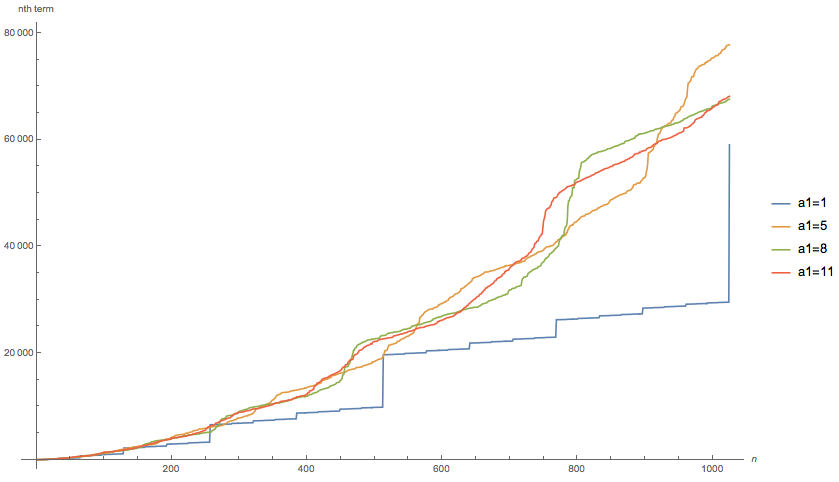
\includegraphics[resolution=140]{plot1.png}
    \caption{Plot of terms in the sequence $A_m$ vs $n$ for different values of $m$}
\end{figure}

\vspace{.5in}

\begin{figure}[!h]
  \centering
    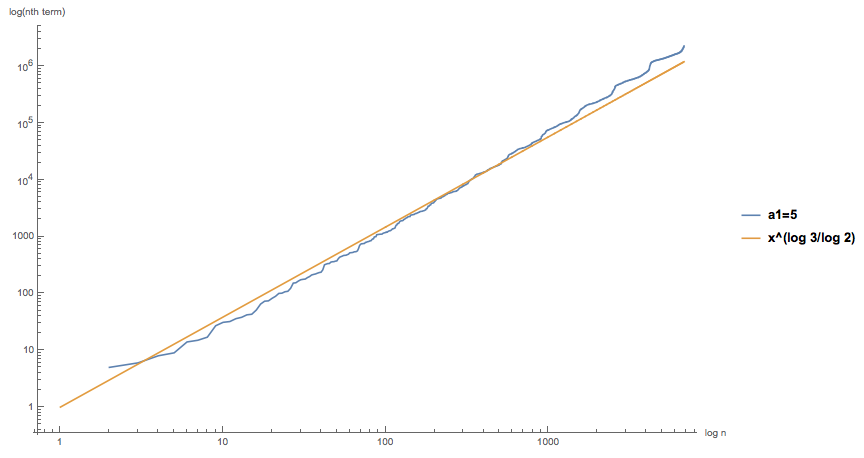
\includegraphics[resolution=140]{plot3.png}
    \caption{Log-log plot of $A_5$ versus $n^{\log_2 3}$}
\end{figure}
\newpage\section{Avoiding solutions to the equation $x + y = z$} \label{sec:diffEquation}

It turns out that the sequence $A$ can be seen as finding terms that avoid a solution to the equation $x + y = 2z$. Interestingly enough, tweaking this equation gives us other sequences with completely different properties.

To begin, we are going to examine the equation $x + y = z$.

We define the modified sequence $A'$ below.

\begin{definition} \label{def:A'}
The sequence $A'$ is defined as the sequence of numbers $a_0, a_1, a_2, \ldots.$ such that $a_0 = 0$, and all subsequent terms $a_{n+1}$ are defined as the least term greater than $a_n$ such that no three distinct terms $x, y, z$ in the sequence $A'$ satisfy the equation $x + y = z$.
\end{definition}

Upon inspection, we see that the first few terms of the sequence are $0, 1, 2, 4, 7, 10, \ldots$. One might therefore predict that every subsequent element $a_n$ for $n \geq 3$ is of the form $3k + 1$, where $k$ is an integer. In fact, we make this statement even stronger.

\begin{theorem}
Every integer of the form $3k + 1$ belongs to the sequence $A'$, and the only integers of the form $3k$ and $3k+2$ that belong to the sequence are $0$ and $2$.
\end{theorem}

\begin{proof}
We will prove this hypothesis by induction.
Our base cases here are $0$, $1$ and $2$ -- clearly they belong to the sequence, because the sequence starts at $0$ and $2 > 0 + 1$.

Now we need to prove the inductive case. Our inductive hypothesis is as follows -- For all numbers $i < k$, if $i \mod 3 = 1$, then $i$ belongs to the sequence $A'$, otherwise $i$ belongs to the sequence only if $i = 0$ or $i = 2$.

Now, we need to prove the inductive hypothesis for $k$. We split this into two cases.

\begin{itemize}

\item \textbf{Case 1:} $k \equiv 1 \mod 3$

We want to prove that when $k \equiv 1 \mod 3$, $k$ belongs to the sequence $A'$. This is easy to see by just looking at remainders modulo 3. By our inductive hypothesis, every number in this sequence is $1$ modulo $3$ except $0$ and $2$. There is no way to obtain a number that is equal to $1$ modulo $3$ by summing two numbers that are also $1$ modulo $3$. In fact, the only way to obtain a number $1$ modulo $3$ given the terms already in the sequence $A'$ is by summing $0$ and a number $1$ modulo $3$, but clearly this does not give a new term in the sequence. Hence we conclude that if $k \equiv 1 \mod 3$, then $k$ must belong to the sequence $A'$.

\item \textbf{Case 2:} $k \not \equiv 1 \mod 3$

Since our base case already contains $0$ and $2$, all we need to do is prove that when $k > 2$ and $k \not \equiv 1 \mod 3$, $k$ cannot belong to the sequence $A'$. This is easy to see since if $k \equiv 0 \mod 3$, we can express $k$ as the sum of $k - 2$ and $2$, which are both part of the sequence ($k - 2$ by the fact that all integers less than $k$ that are congruent to $1$ modulo $3$ belong to the sequence and $2$ by the way the sequence was defined).

Similarly, when $k \equiv 2 \mod 3$ we can express it as the sum of $k -1 $ and $1$, which are both part of the sequence, by our inductive hypothesis.

From this we can conclude that if $k \not \equiv 1 \mod 3$, $k$ does not belong to the sequence $A'$.

\end{itemize}

Since the above two cases hold, we see that the inductive hypothesis holds for $k$ as well, and hence our inductive argument is complete.

\end{proof}

As it turns out, $x+y=z$ and $x+y=2z$ are the only two equations for which we could find a closed form expression for the $n^{th}$ term. We tried several equations of the form $x+y=kz$ where $k>2$, as well as several equations of the form $k_1x+k_2y = (k_1 + k_2)z$ where $k_1 > k_2 \geq 1$. Unfortunately, none of these equations seemed to produce sequences as elegant as the ones presented in this paper.

\emph{Deepak wrote this section. Leon made edits to this section.}

\end{document}